\pdfminorversion=4
\documentclass[aspectratio=169]{beamer}

\mode<presentation>
{
  \usetheme{default}
  \usecolortheme{default}
  \usefonttheme{default}
  \setbeamertemplate{navigation symbols}{}
  \setbeamertemplate{caption}[numbered]
  \setbeamertemplate{footline}[frame number]  % or "page number"
  \setbeamercolor{frametitle}{fg=white}
  \setbeamercolor{footline}{fg=black}
} 

\usepackage[english]{babel}
\usepackage[utf8x]{inputenc}
\usepackage{tikz}
\usepackage{courier}
\usepackage{array}
\usepackage{bold-extra}
\usepackage{minted}
\usepackage[thicklines]{cancel}
\usepackage{fancyvrb}

\xdefinecolor{dianablue}{rgb}{0.18,0.24,0.31}
\xdefinecolor{darkblue}{rgb}{0.1,0.1,0.7}
\xdefinecolor{darkgreen}{rgb}{0,0.5,0}
\xdefinecolor{darkgrey}{rgb}{0.35,0.35,0.35}
\xdefinecolor{darkorange}{rgb}{0.8,0.5,0}
\xdefinecolor{darkred}{rgb}{0.7,0,0}
\definecolor{darkgreen}{rgb}{0,0.6,0}
\definecolor{mauve}{rgb}{0.58,0,0.82}

\title[2019-10-17-pyhep-awkward]{Awkward 1.0}
\author{Jim Pivarski}
\institute{Princeton University -- IRIS-HEP}
\date{October 17, 2019}

\usetikzlibrary{shapes.callouts}

\begin{document}

\logo{\pgfputat{\pgfxy(0.11, 7.4)}{\pgfbox[right,base]{\tikz{\filldraw[fill=dianablue, draw=none] (0 cm, 0 cm) rectangle (50 cm, 1 cm);}\mbox{\hspace{-8 cm}\includegraphics[height=1 cm]{princeton-logo-long.png}\hspace{0.1 cm}\raisebox{0.1 cm}{\includegraphics[height=0.8 cm]{iris-hep-logo-long.png}}\hspace{0.1 cm}}}}}

\begin{frame}
  \titlepage
\end{frame}

\logo{\pgfputat{\pgfxy(0.11, 7.4)}{\pgfbox[right,base]{\tikz{\filldraw[fill=dianablue, draw=none] (0 cm, 0 cm) rectangle (50 cm, 1 cm);}\mbox{\hspace{-8 cm}\includegraphics[height=1 cm]{princeton-logo.png}\hspace{0.1 cm}\raisebox{0.1 cm}{\includegraphics[height=0.8 cm]{iris-hep-logo.png}}\hspace{0.1 cm}}}}}

% Uncomment these lines for an automatically generated outline.
%\begin{frame}{Outline}
%  \tableofcontents
%\end{frame}

% START START START START START START START START START START START START START

\begin{frame}{asdf}
adsf
\end{frame}

\begin{frame}[fragile]{Layer 2: pybind11 of C++}
\vspace{0.5 cm}
\hfill\mbox{\includegraphics[height=4 cm]{awkward-1-0-layers-mini-pybind11.pdf}\hspace{-0.75 cm}}

\scriptsize
\vspace{-4.45 cm}
\begin{columns}
\column{1.1\linewidth}
\begin{minted}{python}
import numpy
import awkward1

content = awkward1.layout.NumpyArray(numpy.arange(10)*1.1)
listA   = awkward1.layout.ListOffsetArray32(
            awkward1.layout.Index32(numpy.array([0, 3, 3, 5, 6, 10])),
            content)
listB   = awkward1.layout.ListOffsetArray32(
            awkward1.layout.Index32(numpy.array([0, 3, 4, 4, 5])),
            listA)
\end{minted}
\begin{uncoverenv}<2->
\begin{minted}{python}
print(awkward1.tolist(listA))
\end{minted}

\vspace{-0.25 cm}
\begin{Verbatim}[commandchars=\\\{\}]
\textcolor{red}{[[0.0, 1.1, 2.2], [], [3.3, 4.4], [5.5], [6.6, 7.7, 8.8, 9.9]]}
\end{Verbatim}
\end{uncoverenv}
\begin{uncoverenv}<3->
\begin{minted}{python}
print(awkward1.tolist(listB))
\end{minted}

\vspace{-0.25 cm}
\begin{Verbatim}[commandchars=\\\{\}]
\textcolor{red}{[[[0.0, 1.1, 2.2], [], [3.3, 4.4]], [[5.5]], [], [[6.6, 7.7, 8.8, 9.9]]]}
\end{Verbatim}
\end{uncoverenv}
\begin{uncoverenv}<4->
\begin{minted}{python}
print(awkward1.tolist(listB[:, ::-1, ::2]))
\end{minted}

\vspace{-0.25 cm}
\begin{Verbatim}[commandchars=\\\{\}]
\textcolor{red}{[[[3.3], [], [0.0, 2.2]], [[5.5]], [], [[6.6, 8.8]]]}    \textcolor{gray}{(old awkward-array can't do this)}
\end{Verbatim}
\end{uncoverenv}
\begin{uncoverenv}<5->
\begin{minted}{python}
print(awkward1.tolist(listB[[0, 0, -1, -1], [0, -1, 0, -1], 1:-1]))
\end{minted}

\vspace{-0.25 cm}
\begin{Verbatim}[commandchars=\\\{\}]
\textcolor{red}{[[1.1], [], [7.7, 8.8], [7.7, 8.8]]}                     \textcolor{gray}{(mixing fancy and basic indexing)}
\end{Verbatim}
\end{uncoverenv}
\end{columns}
\vspace{1 cm}
\end{frame}

\begin{frame}[fragile]{Layer 3: C++ classes}
\vspace{0.5 cm}
\hfill\mbox{\includegraphics[height=4 cm]{awkward-1-0-layers-mini-cpp.pdf}\hspace{-0.75 cm}}

\scriptsize
\vspace{-4.45 cm}
\begin{columns}
\column{1.1\linewidth}
\begin{minted}{c++}
Index32 offsets(6);
offsets.ptr().get()[0] = 0;    offsets.ptr().get()[3] = 5;
offsets.ptr().get()[1] = 3;    offsets.ptr().get()[4] = 6;
offsets.ptr().get()[2] = 3;    offsets.ptr().get()[5] = 10;

auto raw = new RawArrayOf<double>(Identity::none(), 10);
for (int i = 0;  i < 10;  i++) {
  *raw->borrow(i) = 1.1*i;
}
std::shared_ptr<Content> content(raw);
std::shared_ptr<Content> list(new ListOffsetArray32(Identity::none(),
                                                    offsets, content));
\end{minted}
\begin{uncoverenv}<2->
\begin{minted}{c++}
tostring(list);
\end{minted}

\vspace{-0.25 cm}
\begin{Verbatim}[commandchars=\\\{\}]
\textcolor{red}{"[[0, 1.1, 2.2], [], [3.3, 4.4], [5.5], [6.6, 7.7, 8.8, 9.9]]"}
\end{Verbatim}
\begin{minted}{c++}
tostring(list.get()->getitem_range(1, -1));
\end{minted}

\vspace{-0.25 cm}
\begin{Verbatim}[commandchars=\\\{\}]
\textcolor{red}{"[[], [3.3, 4.4], [5.5]]"}
\end{Verbatim}
\begin{minted}{c++}
tostring(list.get()->getitem(slice(new SliceRange(2, Slice::none(), Slice::none()),
                                   new SliceRange(Slice::none(), Slice::none(), -1))));
\end{minted}

\vspace{-0.25 cm}
\begin{Verbatim}[commandchars=\\\{\}]
\textcolor{red}{"[[4.4, 3.3], [5.5], [9.9, 8.8, 7.7, 6.6]]"}
\end{Verbatim}
\end{uncoverenv}
\end{columns}
\vspace{1 cm}
\end{frame}

\begin{frame}[fragile]{Layer 3: Numba models}
\vspace{0.5 cm}
\hfill\mbox{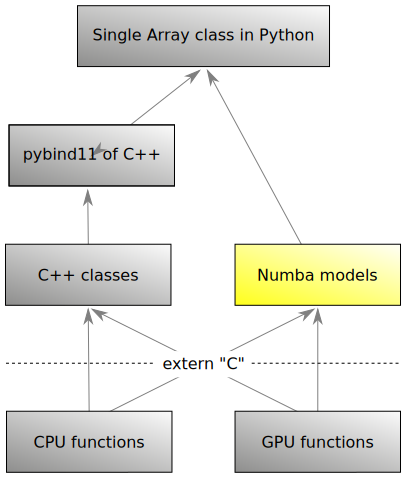
\includegraphics[height=4 cm]{awkward-1-0-layers-mini-numba.pdf}\hspace{-0.75 cm}}

\scriptsize
\vspace{-4.45 cm}
\begin{columns}
\column{1.1\linewidth}
\begin{minted}{python}
import numba

@numba.jit(nopython=True)
def iterate(array):
    out = 0.0
    for subarray in array:               # for loops in a Numba-
        for subsubarray in subarray:     # compiled function are
            for item in subsubarray:     # just as fast as C or C++
                out += item
    return out

print(iterate(listB))
\end{minted}

\vspace{-0.25 cm}
\begin{Verbatim}[commandchars=\\\{\}]
\textcolor{red}{49.5}
\end{Verbatim}
\begin{uncoverenv}<2->
\begin{minted}{python}
@numba.jit(nopython=True)
def slices(array):                       # same slicing works in the compiled environment
    return (array[:, ::-1, ::2],
            array[[0, 0, -1, -1], [0, -1, 0, -1], 1:-1])

one, two = slices(listB)
print(awkward1.tolist(one), awkward1.tolist(two))
\end{minted}

\vspace{-0.25 cm}
\begin{Verbatim}[commandchars=\\\{\}]
\textcolor{red}{[[[3.3], [], [0.0, 2.2]], [[5.5]], [], [[6.6, 8.8]]]}    \textcolor{gray}{(same results as before)}
\textcolor{red}{[[1.1], [], [7.7, 8.8], [7.7, 8.8]]}
\end{Verbatim}
\end{uncoverenv}
\end{columns}
\vspace{1 cm}
\end{frame}

\begin{frame}[fragile]{Layer 4: CPU functions}
\vspace{0.5 cm}
\hfill\mbox{\includegraphics[height=4 cm]{awkward-1-0-layers-mini-cpu.pdf}\hspace{-0.75 cm}}

\scriptsize
\vspace{-4.45 cm}
\begin{columns}
\column{1.1\linewidth}
\begin{uncoverenv}<2->
\begin{minted}{c++}
template <typename C, typename T>
Error awkward_listarray_getitem_next_at(T* tocarry, const C* fromstarts,
          const C* fromstops, int64_t lenstarts, int64_t startsoffset,
          int64_t stopsoffset, int64_t at)
\end{minted}
\end{uncoverenv}

\vspace{-0.35 cm}
\begin{minted}{c++}
{
  for (int64_t i = 0;  i < lenstarts;  i++) {
    int64_t length = fromstops[stopsoffset + i] -
                     fromstarts[startsoffset + i];
    int64_t regular_at = at;
    if (regular_at < 0) {
      regular_at += length;
    }
    if (!(0 <= regular_at  &&  regular_at < length)) {
      return failure("index out of range", i, at);
    }
    tocarry[i] = fromstarts[startsoffset + i] + regular_at;
  }
  return success();
}
\end{minted}

\vspace{-0.35 cm}
\begin{uncoverenv}<3->
\begin{minted}{c++}
extern "C" {
  Error awkward_listarray32_getitem_next_at_64(int64_t* tocarry, const int32_t* fromstarts,
            const int32_t* fromstops, int64_t lenstarts, int64_t startsoffset,
            int64_t stopsoffset, int64_t at);
\end{minted}
\end{uncoverenv}
\end{columns}
\vspace{1 cm}
\end{frame}

\begin{frame}[fragile]{Layer 3: C++ classes}
\vspace{0.5 cm}
\hfill\mbox{\includegraphics[height=4 cm]{awkward-1-0-layers-mini-cpp.pdf}\hspace{-0.75 cm}}

\scriptsize
\vspace{-4.45 cm}
\begin{columns}
\column{1.1\linewidth}
\begin{minted}{c++}
if (head.get() == nullptr) {
  return shallow_copy();
}

else if (SliceAt* at = dynamic_cast<SliceAt*>(head.get())) {
  std::shared_ptr<SliceItem> nexthead = tail.head();
  Slice nexttail = tail.tail();
  Index64 nextcarry(lenstarts);
  Error err = awkward_listarray32_getitem_next_at_64(
    nextcarry.ptr().get(),
    starts_.ptr().get(),
    stops_.ptr().get(),
    lenstarts,
    starts_.offset(),
    stops_.offset(),
    at->at());
  util::handle_error(err, classname(), id_.get());
  std::shared_ptr<Content> nextcontent = content_.get()->carry(nextcarry);
  return nextcontent.get()->getitem_next(nexthead, nexttail, advanced);
}

else if (SliceRange* range = dynamic_cast<SliceRange*>(head.get())) {
  ...
\end{minted}
\end{columns}
\vspace{1 cm}
\end{frame}

\begin{frame}[fragile]{Layer 3: Numba models}
\vspace{0.5 cm}
\hfill\mbox{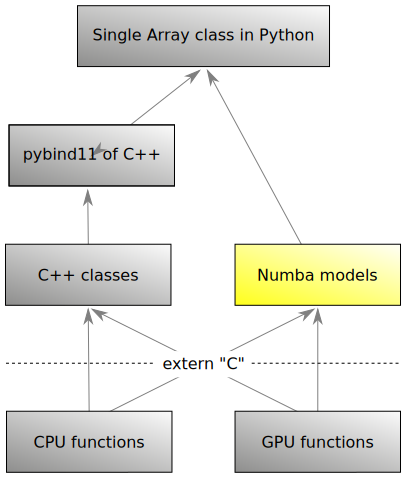
\includegraphics[height=4 cm]{awkward-1-0-layers-mini-numba.pdf}\hspace{-0.75 cm}}

\scriptsize
\vspace{-4.45 cm}
\begin{columns}
\column{1.1\linewidth}
\begin{minted}{python}
if isinstance(headtpe, numba.types.Integer):
  if arraytpe.bitwidth == 64:
    kernel = cpu.kernels.awkward_listarray64_getitem_next_at_64
  elif arraytpe.bitwidth == 32:
    kernel = cpu.kernels.awkward_listarray32_getitem_next_at_64

  nextcarry = util.newindex64(context, builder, numba.int64, lenstarts)
  util.call(context, builder, kernel,
    (util.arrayptr(context, builder, util.index64tpe, nextcarry),
     util.arrayptr(context, builder, arraytpe.startstpe, proxyin.starts),
     util.arrayptr(context, builder, arraytpe.stopstpe, proxyin.stops),
     lenstarts,
     context.get_constant(numba.int64, 0),
     context.get_constant(numba.int64, 0),
     util.cast(context, builder, headtpe, numba.int64, headval)),
    "in {}, indexing error".format(arraytpe.shortname))
  nextcontenttpe = arraytpe.contenttpe.carry()
  nextcontentval = arraytpe.contenttpe.lower_carry(context, builder, arraytpe.contenttpe,
                                           util.index64tpe, proxyin.content, nextcarry)
  return nextcontenttpe.lower_getitem_next(context, builder, nextcontenttpe, tailtpe,
                                           nextcontentval, tailval, advanced)
elif isinstance(headtpe, numba.types.SliceType):
  ...
\end{minted}
\end{columns}
\vspace{1 cm}
\end{frame}



\end{document}
